\question{Câu 12}

 Cho mạch điện như ở Hình 12a, OPAMP được cấp nguồn có $V_{OH} = 3.3\,\textsf{V}$, $V_{OL} =  -3\,\textsf{V}$. Các điện trở được chọn $R_{1} = 2\,\textsf{k}\Omega$, $R_{2} = 5\,\textsf{k}\Omega$ và $R_{3} = 4\,\textsf{k}\Omega$. Cho dạng sóng $V_{i}(t)$ ở hình 12b.
 
 \begin{minipage}{.5\linewidth}
 	\begin{figure}[H]
 		\centering
 		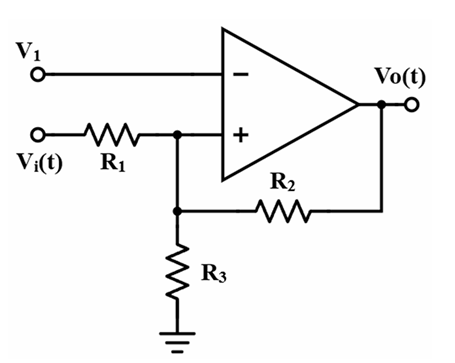
\includegraphics[width=\linewidth]{./my-chapters/my-images/Question12/debai_12a.png}
 		\caption*{Hình 12a.}
 	\end{figure}
 \end{minipage}
 \begin{minipage}{.5\linewidth}
 	\begin{figure}[H]
 		\centering
 		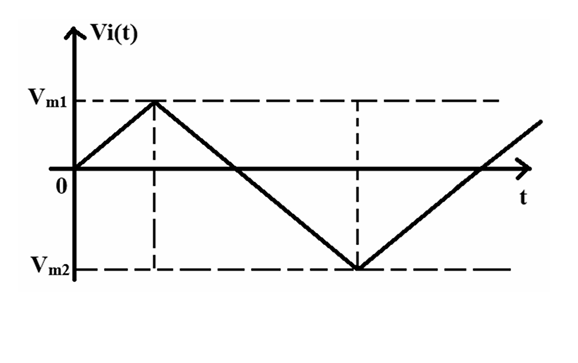
\includegraphics[width=\linewidth]{./my-chapters/my-images/Question12/debai_12b.png}
 		\caption*{Hình 12b.}
 	\end{figure}
 \end{minipage}
 
 \answer{a}{Vẽ dạng sóng ngõ ra $V_{o}$ trong trường hợp $V_{1} = 2\,\textsf{V}$, $V_{m1} = 2\,\textsf{V}$, $V_{m2} = -3\,\textsf{V}$.}
%\[
%V1 = 2V , Vm1 =2 V, Vm2 =-3V
%\]
\[
\dfrac{V_{in}-V_{+}}{R1} = \dfrac{V_{+}\ }{R_{3}} + \dfrac{V_{+}-V_{o}}{R_{2}}
\]
\[
\Rightarrow V_{+} = R_{1}//R_{2}//R_{3}\left(\dfrac{V_{in}}{R_{1}}\ +\dfrac{V_{o}}{R_{2}}\right) \\ [6pt]
\Rightarrow  V_{+} = \ \dfrac{10V_{in}}{19}\ +\dfrac{4V_{o}}{19}\
\]

Khi $V_{o}$ đang ở mức thấp để chuyển sang mức cao  $\Rightarrow V_{+} > 2 $

\[
\Rightarrow  \ \dfrac{10V_{in}}{19}\ +\dfrac{4V_{OL}}{19}\  > 2  \Rightarrow   V_{in} > 5 \,\textsf{V}
\]

Khi $V_{o}$ đang ở mức cao để chuyển sang mức cao  $\Rightarrow V_{+} < 2 $

\[
\Rightarrow  \ \dfrac{10V_{in}}{19}\ +\dfrac{4V_{OH}}{19}\  <  2  \Rightarrow   V_{in} < 2.48 \,\textsf{V}
\]

\begin{figure}[H]
	\centering
	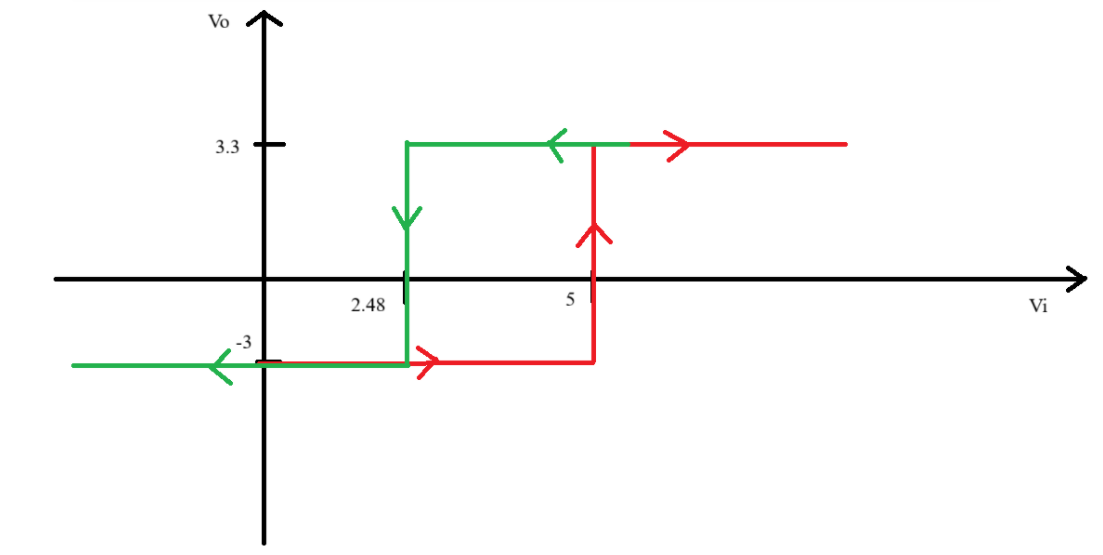
\includegraphics[width=.9\linewidth]{./my-chapters/my-images/Question12/C12_Hình1.png}
	\caption{Đồ thị $V_{o}$ theo $V_{i}$.}
\end{figure}

Với $V_{m1} = 2\,\textsf{V}$, $V_{m2} = -3\,\textsf{V}$, $V_{o}$ luôn ở mức thấp $\Rightarrow V_{o} = V_{OL} = -3\,\textsf{V}$

\begin{figure}[H]
	\centering
	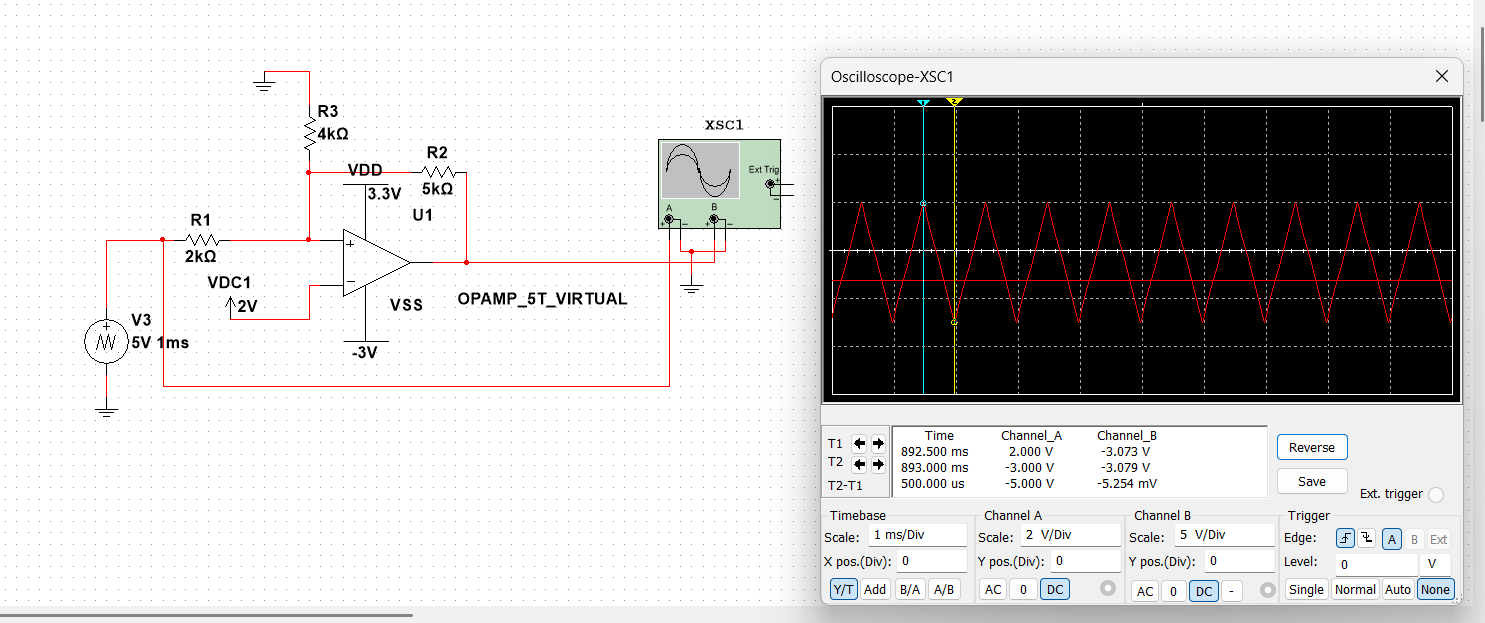
\includegraphics[width=.8\linewidth]{./my-chapters/my-images/Question12/C12_Hình2.png}
	\caption{Mô phỏng Multisim.}
\end{figure}

\answer{b}{Vẽ dạng sóng ngõ ra $V_{o}$ trong trường hợp $V_{1} = 4\,\textsf{V}$, $V_{m1} = 1\,\textsf{V}$, $V_{m2} = -3\,\textsf{V}$.}

Khi $V_{o}$ đang ở mức thấp để chuyển sang mức cao $\Rightarrow V_{+} > 4 $
\[\Rightarrow \dfrac{10V_{in}}{19} +\dfrac{4V_{OL}}{19} > 4 \Rightarrow V_{in} > 8.8 \,\textsf{V}\]
Khi $V_{o}$ đang ở mức cao để chuyển sang mức thấp $\Rightarrow V_{+} < 4 $
\[\Rightarrow \dfrac{10V_{in}}{19} +\dfrac{4V_{OH}}{19} < 4 \Rightarrow V_{in} > 6.28 \,\textsf{V}\]

\begin{figure}[H]
	\centering
	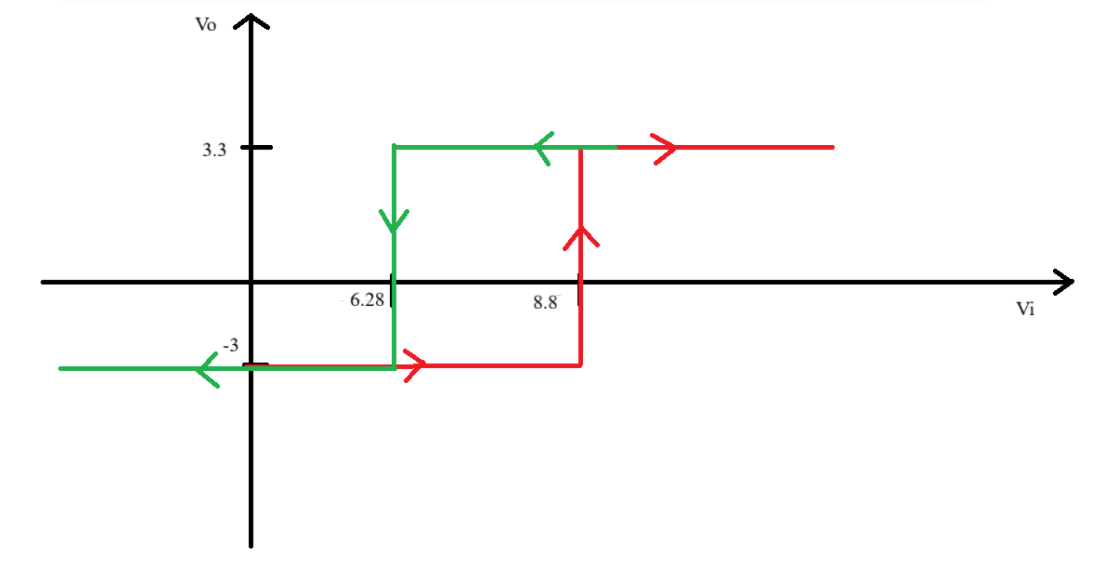
\includegraphics[width=.9\linewidth]{./my-chapters/my-images/Question12/C12_Hình3.png}
	\caption{Đồ thị $V_{o}$ theo $V_{i}$.}
\end{figure}

Với $V_{m1} = 1\,\textsf{V}$, $V_{m2} = -3\,\textsf{V}$, $V_{o}$ luôn ở mức thấp $\Rightarrow V_{o} = V_{OL} = -3\,\textsf{V}$

\begin{figure}[H]
	\centering
	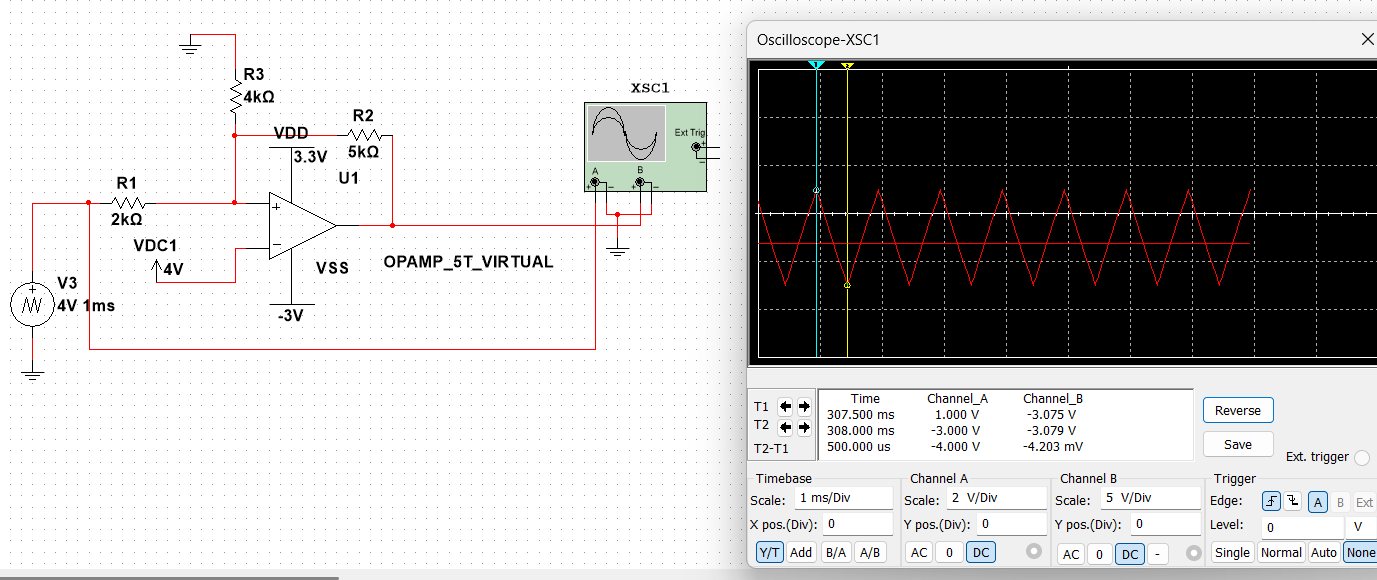
\includegraphics[width=.8\linewidth]{./my-chapters/my-images/Question12/C12_Hình4.png}
	\caption{Mô phỏng Multisim.}
\end{figure}